\section{直线的基本概念}

\begin{definition}[斜截式]
    已知斜率 $k$，已知截距 $b$，其标准方程为 $y=kx+b$，其中 $k$ 是存在的。

    \begin{tips}
        注意斜率的取值范围应该是 $(-\infty, +\infty)$
    \end{tips}

\end{definition}

\begin{theorem}[两点间的斜率公式]
    已知两点 $A(x_1, y_1)$ 和 $B(x_2, y_2)$，则直线 $AB$ 的斜率为 $k = \frac{y_2 - y_1}{x_2 - x_1}$，其中 $x_2 \neq x_1$.
\end{theorem}

\begin{example}
    求两点之间形成的斜率：
    \begin{itemize}
        \item 求点 $(3,-4)$ 和点 $(1,2)$ 两点形成的斜率。
        \item 求点 $(m, 2)$ 和点 $(m-2, 1)$ 两点形成的斜率。
    \end{itemize}
\end{example}

\v{2em}

\begin{theorem}[平面上的点的约束关系]
    $(x,y)$ 是被约束的，所以只要给出一个 $f(x,y)$ 就能描述这个点的轨迹。
\end{theorem}

\begin{example}
    请说出 $3y-x+6=0$ 的点的约束关系。
\end{example}

\v{2em}

\begin{definition}[直线的倾斜角]
    直线的倾斜角 $\theta$ 是指直线与 $x$ 轴正方向之间的夹角，满足 $\tan \theta = k$，其中 $k$ 是直线的斜率。

    \begin{center}
        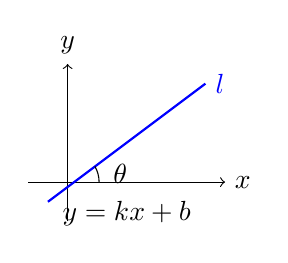
\begin{tikzpicture}[scale=0.5]
            % 绘制坐标轴
            \draw[->] (-1,0) -- (4,0) node[right] {$x$};
            \draw[->] (0,-1) -- (0,3) node[above] {$y$};

            \draw[thick, blue] (-0.5,-0.5) -- (3.5,2.5) node[right] {$l$};
            \draw (0.8,0) arc (0:30:0.8) node[midway, right=2pt] {$\theta$};
            \node at (1.5,-0.8) {$y = kx + b$};
        \end{tikzpicture}
    \end{center}

    \begin{tips}
        直线的倾斜角的取值范围应为 $[0, \pi)$，
    \end{tips}
\end{definition}

\begin{example}
    直线 $l_1: x+5=0$ 与直线 $l_2: 3 x+\sqrt{3} y+2=0$ 的夹角的大小为 \underline{$\qquad$}.
\end{example}

\v{4em}

\begin{example}
    直线 $l$ 的方程为 $x-y \cos \theta+2=0$ ，则直线 $l$ 的倾斜角 $\alpha$ 的取值范围是（ \quad）
    \begin{tasks}(4)
        \task $[0, \pi]$
        \task $\left[\frac{\pi}{4}, \frac{\pi}{2}\right]$
        \task $\left[\frac{\pi}{4}, \frac{3 \pi}{4}\right]$
        \task $\left[\frac{\pi}{4}, \frac{\pi}{2}\right) \cup\left(\frac{\pi}{2}, \frac{3 \pi}{4}\right]$
    \end{tasks}
\end{example}

\v{4em}

\begin{example}
    已知两点 $A(a, 3), B(1,-2)$ ，若直线 $A B$ 的倾斜角为 $135^{\circ}$ ，则 $a$ 的值为（\quad）
    \begin{tasks}(4)
        \task -6
        \task  6
        \task -4
        \task  4
    \end{tasks}
\end{example}

\vspace{2em}

\begin{theorem}[倾斜角与斜率的关系]
    直线的倾斜角 $\alpha$ 的范围是 $[0, \pi)$。斜率 $k = \tan\alpha$。
    \begin{enumerate}
        \item 当 $\alpha \in [0, \pi/2)$ 时，$k \ge 0$ 且 $k$ 随 $\alpha$ 增大而增大；
        \item 当 $\alpha \in (\pi/2, \pi)$ 时，$k < 0$ 且 $k$ 随 $\alpha$ 增大而增大。
    \end{enumerate}
\end{theorem}

\begin{example}
    直线 $l_1, l_2, l_3$ 的斜率分别为 $k_1, k_2, k_3$ ，倾斜角分别为 $\alpha_1, \alpha_2, \alpha_3$ ，则下列选项正确的是（\hspace{2em}）

    \begin{figure} [H]
        \centering
        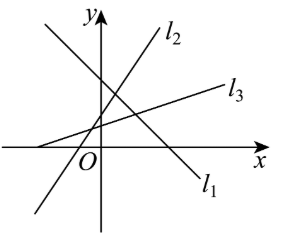
\includegraphics[width=0.15\textwidth]{chapters/linear-circle/images/直线与圆的基本概念/img-20250707161548.png}
    \end{figure}

    \begin{tasks}(4)
        \task $k_1<k_3<k_2$
        \task $k_3<k_2<k_1$
        \task $\alpha_1<\alpha_3<\alpha_2$
        \task $\alpha_3<\alpha_2<\alpha_1$
    \end{tasks}
\end{example}

\begin{theorem}[两条直线之间的夹角公式]
    已知两条直线 $l_1: y = k_1 x + b_1$ 和 $l_2: y = k_2 x + b_2$，则它们之间的夹角 $\theta$ 满足 $\tan \theta = \left| \frac{k_1 - k_2}{1 + k_1 k_2} \right|$，其中 $k_1 k_2 \neq -1$.
\end{theorem}

\begin{example}
    若直线 $l_1, l_2$ 的斜率是方程 $x^2+x-6=0$ 的两根，则这两条直线的夹角为（ \qquad）
    \begin{tasks}(4)
        \task $\frac{\pi}{4}$
        \task $\frac{\pi}{6}$
        \task $\frac{\pi}{3}$
        \task $\frac{\pi}{2}$
    \end{tasks}
\end{example}

\v{4em}

\begin{example}
    已知直线过点 $P(-4,1)$ ，且与直线 $m: 3 x-y+1=0$ 的夹角为 $\arccos \frac{3 \sqrt{10}}{10}$ ，求直线 $l$ 的方程．
\end{example}

\v{4em}

\begin{definition}[一般式]
    已知 $A, B$ 不同时为 $0$，其标准方程为 $Ax+By+C=0$.

    一般式非常通用，可以直接表示任何直线（不需要讨论斜率不存在的情况）。
\end{definition}

\begin{example}
    直线 $x-\sqrt{3} y+1=0$ 的一个方向向量是（\quad ）。
    \begin{tasks}(4)
        \task $(1, \sqrt{3})$
        \task $(\sqrt{3}, 1)$
        \task $(1, -\sqrt{3})$
        \task $(-\sqrt{3}, 1)$
    \end{tasks}
\end{example}

\v{1em}

\begin{definition}[两点式]
    已知两点 $A(x_1, y_1)$ 和 $B(x_2, y_2)$，则直线 $AB$ 的方程为 $\frac{y-y_1}{y_2-y_1} = \frac{x-x_1}{x_2-x_1}$，其中 $x_2 \neq x_1$ 且 $y_2 \neq y_1$.
\end{definition}

\begin{example}
    \begin{itemize}
        \item 已知点 $A(1,2)$ 和点 $B(3,4)$，求直线 $AB$ 的方程。
        \item 求经过两点 $A(2,m)$ 和 $B(n,3)$ 的直线方程。
    \end{itemize}
\end{example}

\v{2em}

\begin{definition}[截距式]
    已知 $x, y$ 轴上的截距 $a, b$ 且 $ab \neq 0$，其标准方程为 $\frac{x}{a} + \frac{y}{b} = 1$。

    其中直线既不能垂直于 $x$ 轴，也不能垂直于 $y$ 轴，且不过原点。
\end{definition}

\begin{example}
    求过点 $(4,3)$ 且在两坐标轴上截距相等的直线 $l$ 的方程。
\end{example}

\begin{solution}
    设直线在 $x$ 轴、 $y$ 轴上的截距分别为 $a, b$ ．

    （1）当 $a \neq 0, b \neq 0$ 时，设 $l$ 的方程为 $\frac{x}{a}+\frac{y}{b}=1$. \\
    $\because$ 点 $(4,-3)$ 在直线上，$\therefore \frac{4}{a}-\frac{3}{b}=1$ ，
    若 $a=b$ ，则 $a=b=1$ ，直线方程为 $x+y-1=0$ ．

    （2）当 $a=b=0$ 时，直线过原点，且过点 $(4,-3)$. \\
    $\therefore$ 直线的方程为 $3 x+4 y=0$ ．
    综上知，所求直线方程为 $x+y-1=0$ 或 $3 x+4 y=0$ ．
\end{solution}

\begin{warning}
    在坐标轴上截距相等，有可能都为 $0$，即一条过原点的直线也会满足这个条件。
\end{warning}

\subsection{多种直线表达式的回顾}
\begin{center}
    \begin{tabular}{|c|c|c|c|}
        \hline
        \textbf{名称} & \textbf{已知条件}                                             & \textbf{标准方程}                                   & \textbf{使用范围}            \\
        \hline
        点斜式         & 斜率 $k$, 直线上一点 $(x_0,y_0)$                                 & $y-y_0 = k(x-x_0)$                              & $k$ 存在                   \\
        \hline
        斜截式         & 斜率 $k$, $y$ 轴截距 $b$                                       & $y=kx+b$                                        & $k$ 存在                   \\
        \hline
        两点式         & $(x_1, y_1)$, $(x_2, y_2)$ ($x_1 \neq x_2, y_1 \neq y_2$) & $\frac{y-y_1}{y_2-y_1} = \frac{x-x_1}{x_2-x_1}$ & 直线不能垂直于 $x$、$y$ 轴        \\
        \hline
        截距式         & $x,y$ 轴上的截距 $a,b$ ($ab \neq 0$)                           & $\frac{x}{a} + \frac{y}{b} = 1$                 & 直线不能垂直于 $x$、$y$ 轴, 且不过原点 \\
        \hline
        一般式         & $A, B$ 不同时为 $0$                                           & $Ax+By+C=0$                                     & 通用                       \\
        \hline
    \end{tabular}
\end{center}

\begin{problem}
求下列直线方程：

（1）若直线 $l$ 经过点 $A(2,-1), B(2,7)$ ，则直线 $l$ 的方程为 \underline{$\qquad$}.

（2）若点 $P(3, m)$ 在过点 $A(2,-1), B(-3,4)$ 的直线上，则 $m=$ \underline{$\qquad$}.
\end{problem}

\v{4em}

\section{直线相关的题型}

\subsection{直线和线段有交点}

\begin{theorem}
    可以直接求端点的斜率出来，也可以用线性规划的知识来解决。
\end{theorem}

\begin{example}
    已知直线 $k x-y+2=0$ 和以 $M(3,-2), ~ N(2,5)$ 为端点的线段相交，则实数 $k$ 的取值范围为（ ）
    A．$\left(-\infty,-\frac{4}{3}\right]$
        B．$\left[\frac{3}{2},+\infty\right)$
    C．$\left[-\frac{4}{3}, \frac{3}{2}\right]$
    D．$\left(-\infty, \frac{4}{3}\right] \cup\left[\frac{3}{2},+\infty\right)$
\end{example}

\v{4em}

\begin{example}
    已知点 $A(2,3), ~ B(3,-1)$ ，若直线 $l$ 过点 $P(0,1)$ 且与线段 $A B$ 相交，则直线 $l$ 的斜率 $k$ 的取值范围是（\qquad）
    \begin{tasks}(4)
        \task $k \leq-\frac{2}{3}$ 或 $k \geq 1$
        \task $k \leq-\frac{2}{3}$ 或 $0 \leq k \leq 1$
        \task $-\frac{2}{3} \leq k \leq 0$ 或 $k \geq 1$
        \task $-\frac{2}{3} \leq k \leq 1$
    \end{tasks}
\end{example}


\subsection{点到直线的距离公式}

\begin{theorem}[点到直线的距离与圆的几何性质]
    求圆上动点与固定两点构成三角形面积的最值问题，通常转化为求圆上动点到该固定两点所在直线的距离的最值问题。其最小（大）距离等于圆心到直线的距离减（加）去半径。
\end{theorem}
\begin{example}
    已知两点 $A(-1,0), ~ B(0,2)$ ，点 $P$ 是圆 $(x-2)^2+y^2=1$ 上任意一点，则 $\triangle P A B$ 面积的最小值是（ \hspace{2em} ）
    \begin{tasks}(4)
        \task $\sqrt{5}$
        \task $2$
        \task $3+\frac{\sqrt{5}}{2}$
        \task $3-\frac{\sqrt{5}}{2}$
    \end{tasks}
\end{example}




\subsection{多选题}
\begin{theorem}[弦长公式的应用]
    利用弦长 $L=2\sqrt{3}$ 和半径 $r=2$，根据公式 $L=2\sqrt{r^2-d^2}$ 求出圆心到直线的距离 $d$。再利用点到直线的距离公式建立关于斜率 $k$ 的方程，解出 $k$ 的值，最后转换为倾斜角。
\end{theorem}
\begin{example}
    直线 $y=k x+3$ 被圆 $(x-2)^2+(y-3)^2=4$ 截得的弦长为 $2 \sqrt{3}$ ，则直线的倾斜角可能为（ \hspace{2em} ）
    \begin{tasks}(4)
        \task $\frac{5 \pi}{6}$
        \task $\frac{\pi}{3}$
        \task $\frac{2 \pi}{3}$
        \task $\frac{\pi}{6}$
    \end{tasks}
\end{example}

\vspace{4em}

\begin{theorem}[直线系与弦长范围]
    直线 $m(x-1) - y + 1 = 0$ 恒过定点 $(1,1)$。由于定点在圆内，直线与圆恒相交。弦长最大值为直径 $4$，最小值为过定点且与定点和圆心连线垂直的弦。计算出最短弦长后即可确定弦长的取值范围。
\end{theorem}
\begin{example}
    直线 $m x-y+1-m=0$ 与圆 $x^2+y^2=4$ 相交，则弦长可能为（ \hspace{2em} ）
    \begin{tasks}(4)
        \task $2$
        \task $3$
        \task $\sqrt{10}$
        \task $5$
    \end{tasks}
\end{example}

\vspace{4em}

\begin{theorem}[圆与圆的位置关系及综合应用]
    A. 直接观察圆 $C_2$ 方程判断半径。B. 比较圆心距与半径和，判断两圆位置关系。C. $|PM|+|PN|$ 的最小值模型，涉及点到圆的距离，需要利用轴对称。D. 过点 $P$ 的切线长公式为 $|PC_1|^2 - r_1^2$，求其最小值需找到使 $|PC_1|$ 最小的点 $P$。
\end{theorem}
\begin{example}
    已知动点 $M, N$ 分别在圆 $C_1:(x-1)^2+(y-2)^2=1$ 和 $C_2:(x-3)^2+(y-4)^2=3$ 上，动点 $P$ 在 $x$ 轴上，则（ \hspace{2em} ）
    \begin{tasks}(4)
        \task 圆 $C_2$ 的半径为 3
        \task 圆 $C_1$ 和圆 $C_2$ 相离
        \task $|P M|+|P N|$ 的最小值为 $2 \sqrt{10}$
        \task 过点 $P$ 做圆 $C_1$ 的切线，则切线长最短为 $\sqrt{3}$
    \end{tasks}
\end{example}

\vspace{4em}

\subsection{多选题}
\begin{theorem}[圆的性质综合判断]
    A. 将圆方程配方为标准式判断半径。B. 将点坐标代入圆方程的左边，判断其值与 $0$ 的关系来确定点与圆的位置。C. 两圆方程作差求公共弦方程。D. 判断圆心距与半径和、差的关系。
\end{theorem}
\begin{example}
    已知 $C: x^2+y^2-6 x=0$ ，则下述正确的是（ \hspace{2em} ）
    \begin{tasks}(4)
        \task 圆 $C$ 的半径 $r=3$
        \task 点 $(1,2 \sqrt{2})$ 在圆 $C$ 的内部
        \task 圆 $C$ 与圆 $x^2+y^2+2 x+4 y-6=0$ 的公共弦所在直线方程为 $4 x+2 y-3=0$
        \task 圆 $C':(x+1)^2+y^2=4$ 与圆 $C$ 相交
    \end{tasks}
\end{example}

\vspace{4em}


\subsection{填空题}
\begin{theorem}[弦长公式与韦达定理]
    联立直线与圆的方程，消元后得到一元二次方程。利用弦长公式 $|MN| = \sqrt{1+k^2}|x_M-x_N|$ 以及韦达定理计算 $|MN|$。利用韦达定理和向量点积坐标公式 $\overrightarrow{OM} \cdot \overrightarrow{ON} = x_M x_N + y_M y_N$ 计算点积。
\end{theorem}
\begin{example}
    已知直线 $y=x+4$ 与圆 $C:(x-1)^2+(y-3)^2=8$ 交于 $M, ~ N$ 两点，$O$ 为坐标原点，则 $|M N|=$ $\qquad$ , $\overrightarrow{O M} \cdot \overrightarrow{O N}=$ $\qquad$ ．
\end{example}

\vspace{4em}


\subsection{解答题}
\begin{theorem}[待定系数法求圆的方程与弦长公式]
    \begin{itemize}
        \item[(1)] 利用圆过两点及圆心在某直线上这三个条件，可以通过解方程组（设圆心坐标 $(a,b)$，利用圆心到两定点距离相等及圆心满足直线方程）来确定圆的方程。
        \item[(2)] 利用点到直线的距离公式求出圆心到弦的距离 $d$，再结合弦长公式 $L=2\sqrt{r^2-d^2}$ 建立关于直线参数的方程求解。
    \end{itemize}
\end{theorem}
\begin{example}
    圆 $C$ 过 $(0,3) 、(4,5)$ 两点，且圆心 $C$ 在直线 $x-y+8=0$ 上．
    \begin{itemize}
        \item[（1）] 求圆 $C$ 的方程；
        \item[（2）] 若直线 $l$ 在 $x$ 轴上的截距是 $y$ 轴上的截距的 2 倍，且被圆 $C$ 截得的弦长为 6 ，求直线 $l$ 的方程。
    \end{itemize}
\end{example}

\vspace{4em}


\subsection{解答题}
\begin{theorem}[圆的方程与位置关系]
    \begin{itemize}
        \item[(1)] 设圆心坐标为 $(a, 1-a)$，利用圆心到 $P, Q$ 两点的距离相等建立关于 $a$ 的方程，求出圆心和半径，得到圆的方程。
        \item[(2)] 以 $AB$ 为直径的圆过原点，等价于 $OA \perp OB$，即 $\overrightarrow{OA} \cdot \overrightarrow{OB} = 0$。设交点坐标，联立直线与圆的方程，利用韦达定理求解。
    \end{itemize}
\end{theorem}
\begin{example}
    已知圆 $C$ 经过 $P(4,-2), Q(-1,3)$ 两点，且圆心 $C$ 在直线 $x+y-1=0$ 上．
    \begin{itemize}
        \item[（1）] 求圆 $C$ 的方程；
        \item[（2）] 若直线 $l: y=-x+m$ 与圆 $C$ 交于点 $A, B$ ，且以线段 $A B$ 为直径的圆经过坐标原点，求直线 $l$ 的方程．
    \end{itemize}
\end{example}

\vspace{4em}

\subsection{解答题}
\begin{theorem}[垂径定理与韦达定理]
    \begin{itemize}
        \item[(1)] 弦的中点 $M$、圆心 $C$、原点 $O$ 构成的直线 $CM$ 与弦 $PQ$ 垂直。利用两直线垂直斜率之积为 $-1$ 的关系，可以求出中点 $M$ 的坐标。
        \item[(2)] 条件 $OP \perp OQ$ 意味着 $\overrightarrow{OP} \cdot \overrightarrow{OQ} = 0$。设 $P(x_1, y_1), Q(x_2, y_2)$，则 $x_1x_2 + y_1y_2 = 0$。联立直线与圆的方程，利用韦达定理建立关于参数 $m$ 的方程求解。
    \end{itemize}
\end{theorem}
\begin{example}
    设 $O$ 是坐标原点，直线 $x+2 y-3=0$ 与圆 $C: x^2+y^2+x-6 y+m=0$ 交于 $P, Q$ 两点．
    \begin{itemize}
        \item[（1）] 求线段 $P Q$ 中点 $M$ 的坐标；
        \item[（2）] 若 $O P \perp O Q$ ，求该圆的面积．
    \end{itemize}
\end{example}

\vspace{4em}

\subsection{解答题}
\begin{theorem}[垂径定理与向量定值问题]
    \begin{itemize}
        \item[(1)] 弦 $MN$ 的中点 $Q$ 满足 $AQ \perp MN$。利用两直线垂直的斜率关系可以求出点 $Q$ 的轨迹方程，再与直线 $l$ 的方程联立求解。
        \item[(2)] 分别用含斜率 $k$ 的代数式表示出点 $P$ 和点 $Q$ 的坐标，然后计算向量点积 $\overrightarrow{B P} \cdot \overrightarrow{B Q}$，化简表达式以判断其是否为定值。
    \end{itemize}
\end{theorem}
\begin{example}
    已知斜率为 $k\left(k \neq-\frac{1}{2}\right)$ 的直线 $l$ 过点 $B(-2,0)$ ，圆 $A:(x+1)^2+(y-2)^2=20$ 与 $l$ 交于 $M, N$ 两点，线段 $M N$ 中点是 $Q$
    \begin{itemize}
        \item[（1）] 若 $k=1$ ，求 $Q$ 坐标
        \item[（2）] 若直线 $l_1: x+2 y+7=0$ 与直线 $l$ 交点是 $P$ ，那么 $\overrightarrow{B P} \cdot \overrightarrow{B Q}$ 是否为定值？如果是，求出定值；如果不是，说明理由．
    \end{itemize}
\end{example}

\vspace{4em}

\subsection{选择题}


\subsection{选择题}
\begin{theorem}[两直线夹角公式]
    设两直线 $l_1, l_2$ 的斜率分别为 $k_1, k_2$，则它们之间的夹角 $\theta$ (锐角或直角) 满足公式 $\tan\theta = \left|\frac{k_2 - k_1}{1 + k_1 k_2}\right|$。
\end{theorem}
\begin{example}
    直线 $2 x-3 y+1=0$ 与 $x+5 y-10=0$ 的夹角为（\hspace{2em}）。
    \begin{tasks}(4)
        \task $\frac{\pi}{6}$
        \task $\frac{\pi}{4}$
        \task $\frac{\pi}{3}$
        \task $\frac{2 \pi}{3}$
    \end{tasks}
\end{example}

\vspace{4em}

\subsection{选择题}
\begin{theorem}[斜率的几何意义]
    过定点 $P$ 的直线与线段 $AB$ 相交，则该直线的斜率 $k$ 必介于直线 $PA$ 和 $PB$ 的斜率之间（包含边界）。通过计算 $k_{PA}$ 和 $k_{PB}$ 即可确定 $k$ 的取值范围。
\end{theorem}
\begin{example}
    已知点 $A(2,3), ~ B(3,-1)$ ，若直线 $l$ 过点 $P(0,1)$ 且与线段 $A B$ 相交，则直线 $l$ 的斜率 $k$ 的取值范围是（\hspace{2em}）
    \begin{tasks}(4)
        \task $k \leq-\frac{2}{3}$ 或 $k \geq 1$
        \task $k \leq-\frac{2}{3}$ 或 $0 \leq k \leq 1$
        \task $-\frac{2}{3} \leq k \leq 0$ 或 $k \geq 1$
        \task $-\frac{2}{3} \leq k \leq 1$
    \end{tasks}
\end{example}

\vspace{4em}

\subsection{选择题}
\begin{theorem}[斜率的几何意义]
    表达式 $\frac{y-y_0}{x-x_0}$ 表示动点 $(x,y)$ 与定点 $(x_0, y_0)$ 连线的斜率。本题中 $\frac{y}{x-3}$ 即为线段 $AB$ 上的点 $P(x,y)$ 与定点 $(3,0)$ 连线的斜率。通过计算定点与线段两端点连线的斜率，即可找到其最大值和最小值。
\end{theorem}
\begin{example}
    已知 $A(2,3), B(-1,2)$ ，若点 $P(x, y)$ 在线段 $A B$ 上，则 $\frac{y}{x-3}$ 的最小值为（\hspace{2em}）
    \begin{tasks}(4)
        \task $1$
        \task $\frac{3}{5}$
        \task -3
        \task $-\frac{1}{2}$
    \end{tasks}
\end{example}

\vspace{4em}

\subsection{选择题}
\begin{theorem}[两直线垂直的条件]
    若两条直线 $l_1, l_2$ 的斜率都存在且不为零，它们相互垂直的充要条件是其斜率之积为-1，即 $k_1 k_2 = -1$。
\end{theorem}
\begin{example}
    已知直线 $l_1$ 过 $A(1,3), B(2,5)$ 两点，且 $l_1 \perp l_2$ ，则直线 $l_2$ 的斜率为（\hspace{2em}）
    \begin{tasks}(4)
        \task $\frac{2}{3}$
        \task $-\frac{2}{3}$
        \task $\frac{1}{2}$
        \task $-\frac{1}{2}$
    \end{tasks}
\end{example}

\vspace{4em}

\subsection{选择题}
\begin{theorem}[点关于直线对称的性质]
    若两点 $P, Q$ 关于直线 $l$ 对称，则：1. 直线 $l$ 经过线段 $PQ$ 的中点。2. 直线 $l$ 与直线 $PQ$ 垂直。根据这些性质可以逐一判断选项的真伪。
\end{theorem}
\begin{example}
    已知 $P(4,5)$ 与 $Q(-2,7)$ 关于直线 $l$ 对称，则下列说法中错误的是（\hspace{2em}）
    \begin{tasks}(4)
        \task 直线 $l$ 过 $P, Q$ 的中点
        \task 直线 $P Q$ 的斜率为 $\frac{1}{3}$
        \task 直线 $l$ 的斜率为 3
        \task 直线 $l$ 的一个方向向量的坐标是 $(1,3)$
    \end{tasks}
\end{example}

\vspace{4em}

\subsection{选择题}
\begin{theorem}[圆的标准方程]
    以线段 $AB$ 为直径的圆，其圆心为 $AB$ 的中点，其半径为 $AB$ 长度的一半。求出圆心坐标 $(a,b)$ 和半径 $r$ 后，即可写出圆的标准方程 $(x-a)^2 + (y-b)^2 = r^2$。
\end{theorem}
\begin{example}
    已知点 $A(1,-1)$ 和点 $B(-1,3)$ ，则以线段 $A B$ 为直径的圆的标准方程为（\hspace{2em}）
    \begin{tasks}(4)
        \task $(x+2)^2+(y-4)^2=5$
        \task $(x+2)^2+(y-4)^2=20$
        \task $x^2+(y-1)^2=5$
        \task $x^2+(y-1)^2=20$
    \end{tasks}
\end{example}

\vspace{4em}

\subsection{多选题}
\begin{theorem}[直线方程的综合辨析]
    需逐一分析各选项：A. 倾斜角为 $90^\circ$ 的直线（垂直于x轴）没有斜率。B. 利用两直线平行（$A_1B_2=A_2B_1$）且不重合的条件判断。C. 此为两点式方程，其适用条件需注意。D. 考虑截距为0和不为0两种情况。
\end{theorem}
\begin{example}
    下列四个选项中，说法错误的是（\hspace{2em}）
    \begin{itemize}
        \item  坐标平面内的任何一条直线均有倾斜角和斜率
        \item  直线 $a x+2 y+6=0$ 与直线 $x+(a-1) y+a^2-1=0$ 互相平行，则 $a=-1$
        \item  过 $\left(x_1, y_1\right),\left(x_2, y_2\right)$ 两点 $\left(x_1 \neq x_2, y_1 \neq y_2\right)$ 的所有直线的方程为 $\frac{y-y_1}{y_2-y_1}=\frac{x-x_1}{x_2-x_1}$
        \item  经过点 $(1,1)$ 且在 $x$ 轴和 $y$ 轴上截距都相等的直线方程为 $x+y-2=0$ ．
    \end{itemize}
\end{example}

\vspace{4em}

\subsection{多选题}
\begin{theorem}[直线方程的性质]
    (1) 利用直线系（定点）的知识判断。(2) 直线在y轴上的截距是当x=0时y的值。(3) 通过斜率 $k=\tan\alpha$ 求解倾斜角。(4) 讨论截距为0和不为0两种情况。
\end{theorem}
\begin{example}
    下列说法正确的是
    \begin{itemize}
        \item[（1）] 直线 $y=a x-2 a+4(a \in \mathrm{R})$ 恒过定点 $(2,4)$
        \item[（2）] 直线 $y+1=3 x$ 在 $y$ 轴上的截距为 1
        \item[（3）] 直线 $x+\sqrt{3} y+1=0$ の倾斜角为 $150^{\circ}$
        \item[（4）] 已知直线 $l$ 过点 $P(2,4)$ ，且在 $x, y$ 轴上截距相等，则直线 $l$ 的方程为 $x+y-6=0$
    \end{itemize}
\end{example}

\vspace{4em}

\subsection{填空题}
\begin{theorem}[倾斜角与斜率]
    直线的斜率 $k$ 与其倾斜角 $\alpha$ 的关系为 $k=\tan\alpha$。已知倾斜角为 $135^\circ$，可直接求出斜率 $k=-1$，代入直线方程的斜率表达式即可求解。
\end{theorem}
\begin{example}
    若直线 $(k+1) x-y+2=0$ 的倾斜角为 $135^{\circ}$ ，则 $k=\qquad$
\end{example}

\vspace{4em}

\subsection{填空题}
\begin{theorem}[点斜式方程]
    先求出已知直线的倾斜角 $\alpha_1$，然后得到所求直线 $l$ 的倾斜角 $\alpha_2 = \alpha_1 / 2$。计算出直线 $l$ 的斜率 $k_2 = \tan\alpha_2$，最后利用点斜式方程 $y-y_0=k(x-x_0)$ 写出结果。
\end{theorem}
\begin{example}
    已知直线 $l$ 经过点 $P(\sqrt{2}, 1)$ ，且倾斜角等于直线 $y=-\sqrt{3} x+3$ 的倾斜角的一半，则直线 $l$ 的点斜式方程为 $\qquad$
\end{example}

\vspace{4em}

\subsection{填空题}
\begin{theorem}[斜率与半角公式]
    设已知直线的倾斜角为 $\alpha$，斜率为 $k_1$，则 $k_1=\tan\alpha$。所求直线的倾斜角为 $\beta = \alpha/2$，斜率为 $k_2 = \tan\beta$。利用正切的半角公式 $\tan\alpha = \frac{2\tan(\alpha/2)}{1-\tan^2(\alpha/2)}$ 建立关于 $k_2$ 的方程并求解，然后写出直线方程。
\end{theorem}
\begin{example}
    若直线过点 $(-2,3)$ ，且倾斜角是直线 $3 x+4 y-5=0$ 的倾斜角的一半，则直线 l 的方程为 $\qquad$
\end{example}

\vspace{4em}

\subsection{填空题}
\begin{theorem}[斜率的几何意义]
    直线 $l$ 过定点 $P$ 并与线段 $AB$ 相交，则直线 $l$ 的斜率范围由 $k_{PA}$ 和 $k_{PB}$ 决定。倾斜角的范围需要根据斜率的正负和单调性进行讨论，注意倾斜角的取值范围是 $[0, \pi)$。
\end{theorem}
\begin{example}
    已知点 $A(-1,3), B(3,2)$ ，过点 $P\left(\frac{3}{2}, \frac{1}{2}\right)$ 的直线 $l$ 与线段 $A B$ 相交，则直线 $l$ 的倾斜角的取值范围为 $\qquad$ ，直线 $l$ 的斜率的取值范围为 $\qquad$ ．
\end{example}

\vspace{4em}

\subsection{解答题}
\begin{theorem}[直线的基本性质]
    \begin{itemize}
        \item[（1）] 将已知点的坐标代入直线方程，即可求出斜率 $k$。再利用 $k=\tan\alpha$ 求倾斜角。
        \item[（2）] 直线在 $x$ 轴上的截距即是令 $y=0$ 时所求得的 $x$ 值。
    \end{itemize}
\end{theorem}
\begin{example}
    已知直线 $l: y=k x+2$ 经过点 $(1,-3)$ ．
    \begin{itemize}
        \item[（1）] 求直线 $l$ 的倾斜角；
        \item[（2）] 求直线 $l$ 在 $x$ 轴上的截距．
    \end{itemize}
\end{example}

\vspace{4em}

\subsection{解答题}
\begin{theorem}[直线系与参数范围]
    \begin{itemize}
        \item[（1）] 将直线方程整理为关于参数 $a$ 的形式 $a(2x-y) + (-3x+y+1) = 0$，令系数同时为零，解方程组即可求得定点坐标。
        \item[（2）] 直线不经过第二象限，意味着其斜率 $k \ge 0$ 且其 $y$ 轴截距 $b \le 0$（或斜率不存在时，$x$ 截距大于等于0）。通过分析斜率和截距与 $a$ 的关系来求解 $a$ 的范围。
        \item[（3）] 写出两截距关于参数 $a$ 的表达式，进而写出面积的表达式，利用基本不等式求其最小值。
    \end{itemize}
\end{theorem}
\begin{example}
    已知直线 $l:(a-1) y=(2 a-3) x+1$ ．
    \begin{itemize}
        \item[（1）] 求证：直线 $l$ 过定点；
        \item[（2）] 若直线 $l$ 不经过第二象限，求实数 $a$ 的取值范围；
        \item[（3）] 若直线 $l$ 与两坐标轴的正半轴围成的三角形面积最小，求 $l$ 的方程．
    \end{itemize}
\end{example}

\vspace{4em}

\subsection{解答题}
\begin{theorem}[直线系与最值问题]
    \begin{itemize}
        \item[（1）] 将方程整理为 $a(x-2) + (x+y-5)=0$ 的形式，解方程组 $\begin{cases} x-2=0 \\ x+y-5=0 \end{cases}$ 即可找到定点。
        \item[（2）] 用参数 $a$ 表示出两截距，进而表示出三角形面积 $S$。利用换元法和基本不等式求 $S$ 的最小值。
        \item[（3）] 将两截距的表达式设为正整数，通过分析表达式的结构和 $a$ 为正整数的条件，求解不定方程。
    \end{itemize}
\end{theorem}
\begin{example}
    设直线 $l$ 的方程为 $(a+1) x+y-5-2 a=0(a \in \mathrm{R})$ ．
    \begin{itemize}
        \item[（1）] 求证：不论 $a$ 为何值，直线必过一定点 $P$ ；
        \item[（2）] 若直线 $l$ 分别与 $x$ 轴正半轴，$y$ 轴正半轴交于点 $A\left(x_A, 0\right), B\left(0, y_B\right)$ ，当 $\Delta A O B$ 面积最小时，求此时的直线方程；
        \item[（3）] 当直线 $l$ 在两坐标轴上的截距均为正整数且 $a$ 也为正整数时，求直线 $l$ 的方程．
    \end{itemize}
\end{example}

\vspace{4em}

% =============================================
% 第三批题目 (来自图片)
% =============================================

\subsection{解答题}
\begin{theorem}[线段垂直平分线与点到直线距离]
    \begin{itemize}
        \item[(1)] 线段的垂直平分线满足两个条件：过线段中点，且与线段所在直线垂直。
        \item[(2)] 一条直线与两相异定点 $A, B$ 的距离相等，意味着该直线或者平行于直线 $AB$，或者经过线段 $AB$ 的中点。
    \end{itemize}
\end{theorem}
\begin{example}
    已知点 $A(1,3), B(5,7)$．
    \begin{itemize}
        \item[(1)] 求线段 $AB$ 垂直平分线所在直线的方程；
        \item[(2)] 若直线 $l$ 过 $(-1,0)$，且点 $A、B$ 到直线 $l$ 的距离相等，求直线 $l$ 的方程．
    \end{itemize}
\end{example}

\vspace{4em}

\subsection{解答题}
\begin{theorem}[直线系与圆的综合应用]
    \begin{itemize}
        \item[(1)] 首先将含参的直线方程整理为 $m(x+2y-5) + (-x+3) = 0$ 的形式，求出其恒过的定点。然后判断该定点与圆的位置关系，若定点在圆内，则直线与圆恒相交。
        \item[(2)] 过圆内一定点的所有弦中，最短的弦是与过该定点的直径垂直的弦。此时，圆心到弦的距离最大，等于圆心与该定点之间的距离。利用弦长公式 $L=2\sqrt{r^2-d^2}$ 即可求出最短弦长。
    \end{itemize}
\end{theorem}
\begin{example}
    已知直线 $l: (m-1)x + 2my - 5m + 3 = 0, m \in \mathrm{R}$ 和圆 $C: (x-2)^2 + (y-1)^2 = 4$．
    \begin{itemize}
        \item[(1)] 证明：圆 $C$ 与直线 $l$ 恒相交；
        \item[(2)] 求直线 $l$ 被圆 $C$ 截得的弦长的最小值．
    \end{itemize}
\end{example}

\subsection{选择题}
\begin{theorem}[抛物线定义与圆的切线长]
    利用圆的切线长公式 $l^2 = |PC|^2 - r^2$ 建立方程，其中 $P$ 为切点，$C$ 为圆心。将点 $P$ 的坐标代入，并结合点 $P$ 在抛物线上满足的方程 $y^2=2px$，解出点 $P$ 的横坐标。最后根据抛物线的定义，点 $P$ 到准线的距离等于 $x_P + p/2$。
\end{theorem}
\begin{example}
    已知点 $P$ 在抛物线 $M: y^2=8 x$ 上，过点 $P$ 作圆 $C:(x-4)^2+y^2=1$ 的切线，若切线长为 $2 \sqrt{6}$ ，则点 $P$ 到 $M$ 的准线的距离为（ ）
    \begin{tasks}(4)
        \task $5$
        \task $6$
        \task $7$
        \task $4 \sqrt{2}$
    \end{tasks}
\end{example}

\vspace{4em}

\subsection{选择题}
\begin{theorem}[圆的切线性质与向量点积]
    由圆的切线性质可知，$PM \perp MC$，其中 $C$ 为圆心，$M$ 为切点。因此 $\triangle PMC$ 是直角三角形。利用向量点积的几何意义，$\overrightarrow{PM} \cdot \overrightarrow{PC} = |\overrightarrow{PM}||\overrightarrow{PC}|\cos\angle MPC = |\overrightarrow{PM}|^2$。问题转化为求 $|PM|^2$ 的最小值。根据切线长公式 $|PM|^2=|PC|^2-r^2$，求 $|PM|$ 的最小值等价于求动点 $P$ 到圆心 $C$ 的距离 $|PC|$ 的最小值。
\end{theorem}
\begin{example}
    在平面直角坐标系 $x O y$ 中，已知圆 $C:(x-1)^2+y^2=4, ~ P$ 为直线 $l: x+y+3=0$ 上的一个动点，过点 $P$ 作圆 $C$ 的切线 $P M$ ，切点为点 $M$ ，当 $|P M|$ 最小时，则 $\overrightarrow{P M} \cdot \overrightarrow{P C}$ 的值为（ ）
    \begin{tasks}(4)
        \task $4$
        \task $\sqrt{2}$
        \task $2$
        \task $3$
    \end{tasks}
\end{example}

\vspace{4em}

\subsection{多选题}
\begin{theorem}[圆与圆的位置关系及最值问题]
    A. 由圆的标准方程 $(x-a)^2+(y-b)^2=r^2$ 直接读出半径。B. 比较圆心距与两半径之和、差判断位置关系。C. $|PM|+|PN|$ 的最小值模型，通常利用轴对称转化为两定点间距离问题，再减去相应半径。D. 过点 $P$ 的切线长公式为 $l^2 = |PC|^2 - r^2$，其最小值取决于 $|PC|$ 的最小值。
\end{theorem}
\begin{example}
    已知动点 $M, N$ 分别在圆 $C_1:(x-1)^2+(y-2)^2=1$ 和 $C_2:(x-3)^2+(y-4)^2=3$ 上，动点 $P$ 在 $x$ 轴上，则（）
    \begin{tasks}(4)
        \task 圆 $C_2$ 的半径为 3
        \task 圆 $C_1$ 和圆 $C_2$ 相离
        \task $|P M|+|P N|$ 的最小值为 $2 \sqrt{10}$
        \task 过点 $P$ 做圆 $C_1$ 的切线，则切线长最短为 $\sqrt{3}$
    \end{tasks}
\end{example}

\vspace{4em}

\subsection{多选题}
\begin{theorem}[直线系与圆的综合应用]
    A. 将直线方程整理为关于参数 $m$ 的形式，解出与 $m$ 无关的定点坐标。B. 令 $x=0$ 求圆与 $y$ 轴的交点，计算弦长。C. 判断定点与圆的位置关系，若定点在圆内，则直线与圆恒相交。D. 过圆内定点的最短弦为与定点和圆心连线垂直的弦。
\end{theorem}
\begin{example}
    已知圆 $C:(x-1)^2+(y-2)^2=25$ ，直线 $l:(2 m+1) x+(m+1) y-7 m-4=0$ ．则下列命题正确的有（ ）
    \begin{tasks}(4)
        \task 直线 $l$ 恒过定点 $(3,1)$
        \task 圆 $C$ 被 $y$ 轴截得的弦长为 $2 \sqrt{6}$
        \task 直线 $l$ 与圆 $C$ 恒相交
        \task 直线 $l$ 被圆 $C$ 截得弦长最短时，直线 $l$ 的方程为 $2 x-y-5=0$
    \end{tasks}
\end{example}

\vspace{4em}

\subsection{填空题}
\begin{theorem}[点到圆的距离与几何意义]
    表达式 $x^2+y^2$ 的几何意义是圆上点 $P(x,y)$ 到坐标原点 $O(0,0)$ 距离的平方。其最大（小）值等于（圆心到原点的距离与半径的和（差））的平方。
\end{theorem}
\begin{example}
    若点 $P(x, y)$ 是圆 $x^2+y^2-2 x+4 y+1=0$ 上任意一点，则 $x^2+y^2$ 的最大值是 $\qquad$ ．
\end{example}

\vspace{4em}

\subsection{解答题}
\begin{theorem}[点到圆的距离最值]
    求解表达式 $(x-a)^2+(y-b)^2$ 的最值，可以将其看作圆上动点 $P(x,y)$ 到定点 $A(a,b)$ 距离的平方。其最大值为 $(|AC|+r)^2$，最小值为 $(|AC|-r)^2$，其中 $C$ 是圆心，$r$ 是半径。
\end{theorem}
\begin{example}
    已知点 $P(x, y)$ 在圆 $C_1: x^2+(y-1)^2=1$ 上运动．求 $(x-2)^2+y^2$ 的最大值与最小值．
\end{example}

\begin{problemset}
    \item 过点 $(-2,0)$ 与圆 $x^2+y^2-6 x=0$ 相切的两条直线的夹角为 $\alpha$ ，则 $\sin \alpha=$ \underline{$\qquad$} ．
    \item 两直线 $y=x-1$ 与 $x-2 y+1=0$ 的夹角为 \underline{$\qquad$} ．（结果用反三角表示）
\end{problemset}

\subsection{练习答案}
\begin{tips}
    \begin{enumerate}
        \item 过点 $(-2,0)$ 与圆 $x^2+y^2-6 x=0$ 相切的两条直线的夹角为 $\alpha$ ，则 $\sin \alpha= \frac{24}{25}$ ．
        \item 两直线 $y=x-1$ 与 $x-2 y+1=0$ 的夹角为 $arctan\frac{1}{3}$
    \end{enumerate}
\end{tips}